\section{旋转建模法}
\subsection{绘制左视图}
\begin{procedure}
\item 设置图层,新建“中心线”和“实线”两个图层,具体设计请参看\ref{sec:dianpian}节的图层设置相关内容。
\item  切换视图为主视图。【视图】菜单中【三维视图】子菜单中的【左视图】。
\item 绘制中心线,其结果如图\ref{fig:dianpiancenterline1}所示。
\begin{lstlisting}
|命令: xline|
|指定点或 [水平(H)/垂直(V)/角度(A)/二等分(B)/偏移(O)]:|
|指定通过点:$@1<0$|
|指定通过点:$@1<90$|
|指定通过:|
|命令:OFFSET|
|当前设置: 删除源=否  图层=源  OFFSETGAPTYPE=0|
|指定偏移距离或 [通过(T)/删除(E)/图层(L)] $<$通过$>$:  42|
|选择要偏移的对象,或 [退出(E)/放弃(U)] $<$退出$>$:|
|指定要偏移的那一侧上的点,或 [退出(E)/多个(M)/放弃(U)] $<$退出$>$:|
|选择要偏移的对象,或 [退出(E)/放弃(U)] $<$退出$>$:
\end{lstlisting}
\item 将图层切换为实线层
\begin{figure}[htbp]
\centering
\subfloat[]{\label{fig:dianpiancenterline1}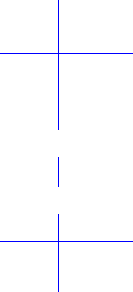
\includegraphics[scale=0.6]{dianpiancenterline1.png}}\hspace{40pt}
\subfloat[]{\label{fig:dianpianleft1}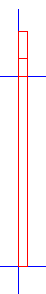
\includegraphics[scale=0.6]{dianpianleft1.png}}
\caption{垫片左视图绘制}
\end{figure}
\item 使用【矩形】命令绘制左视图中的关键特征,其结果如图\ref{fig:dianpianleft1}所示。【矩形】命令的启动方法有:
\begin{itemize}
\item 键盘输入RECTANGLE或REC
\item 点击【绘图】菜单中的【矩形】项。
\item 点击【绘图】工具栏中的【矩形】图标
\includegraphics[scale=0.6]{rectangletool.png}
\end{itemize}
\begin{lstlisting}
|命令: rectang|
|指定第一个角点或 [倒角(C)/标高(E)/圆角(F)/厚度(T)/宽度(W)]:|
|指定另一个角点或 [面积(A)/尺寸(D)/旋转(R)]: @2,52|
|命令: rectang|
|指定第一个角点或 [倒角(C)/标高(E)/圆角(F)/厚度(T)/宽度(W)]:|
|指定另一个角点或 [面积(A)/尺寸(D)/旋转(R)]: @2,4|
|命令: rectang|
|指定第一个角点或 [倒角(C)/标高(E)/圆角(F)/厚度(T)/宽度(W)]:|
|指定另一个角点或 [面积(A)/尺寸(D)/旋转(R)]: @2,26.5|
\end{lstlisting}
\end{procedure}

\endinput